\section{Practical Security}

The theoretical guarantees in the previous sections — that security is guaranteed without needing to trust
the server or the network — all assume that your local computer is completely trusted. This is unavoidable: no matter the fancy encryption schemes you come up with, nothing will help you if your computer comes with a preinstalled backdoor. Nevertheless, while \textbf{we fundamentally cannot eliminate the client-side risk} (no one can), \textit{we can reduce it}. We care about this practical security as much as we care about the theoretical security, and in this section we outline the mitigations we undertake: reducing the attack surface by modularizing and reducing supply chain risk, minimizing bugs by being open source and having an extensive test suite, securing code distribution and updates, and protecting against non-privileged local malware.

Still, we cannot achieve perfect security here, so: \textbf{PLEASE DO NOT USE ANYSPHERE FOR SECURITY-CRITICAL USE CASES ON A COMPUTER YOU DO NOT TRUST}. This is especially true while we are in beta, and may have bugs.

% The Anysphere client is only as strong and secure as the most vulnerable part of our software supply chain. Software supply chains are an increasingly complex (and brittle) part of the software ecosystem because of a large and growing number of direct and transitive dependencies written across the world. 
% The Anysphere client is designed to handle extreme private and critical communication securely, so our team has enforced a high bar of security for the core of our system. We focused on providing practical protection by significantly reducing the attack surface of our client, ensuring safe updates, and protecting against non-privileged software. 

% A note on the client's security, in the context of our threat model: Anysphere trusts its client's devices. 
% In particular, we trust that the local device is running a correct implementation of our protocol, and the computer comes without pre-installed backdoors. 
% Our model is the bare minimum of trust we must assume, and we think this is reasonable given the intense focus of Apple and many other companies on device security. 
% (Put another way, no encryption schemes we can come up with can secure our client inside a compromised computer.)
% And with this context, we will present our measures to reduce the risk of a compromised Anysphere client.


\subsection{Reducing the attack surface: modularity and supply chain risk}

We architected our client to consist of two parts: a UI frontend and a daemon backend, where the daemon backend contains all security-critical code. We sandbox the UI frontend in such a way that it is not allowed to talk to the internet, and let all message sending go through the daemon, which handles the cryptography. That way, even if there are bugs in the UI frontend, or potentially malicious code, there is not much it can do.

\begin{figure*}[htb]
    \centering
    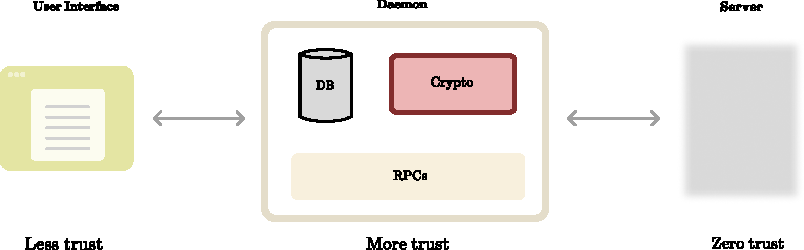
\includegraphics[width=0.8\textwidth]{systemdiagram.pdf}
\caption{System architecture. The user interface and the daemon run on your local computer and require some trust assumptions. The user interface is cut off from the internet, and can only communicate via the daemon, meaning that it needs lower trust assumptions. The crypto module in the daemon requires the highest level of trust, and uses the widely trusted Libsodium library.}
\end{figure*}

We also reduce the attack surface of the daemon itself. In particular, we use C++ instead of other popular languages (Rust, Go, Python), because all other practical languages are significantly more susceptible to supply chain attacks. Our daemon has 4 direct dependencies (Abseil, gRPC, SQLite, Libsodium) and 0 transitive dependencies. A comparable implementation in a language with a package manager would easily use 100s of transitive dependencies. We elaborate more on our choice of C++ in this blog post \todo{Link.}.

\subsection{Minimizing bugs: open source and tests}

\subsection{Code distribution and updates}



\todo{mention that we are NOT a web app. this is critical.}

% We sign everything.

% Maybe we sign everything twice?

% Maybe we have a cold-storage and a hot-storage signing key?

% Do we store a backup key in cold storage that we can use to revoke a version? And people can disi

% \todo{Either understand whether standard OS signing is good enough, or whether we should sign things ourselves.}


\subsection{Updates}

Every update needs to be signed. In fact, it needs to be signed twice: Arvid holds one key, and Sualeh holds one key. Both signatures must be present for the local client to accept the update.

We implement our own signature check. Many popular frameworks have built-in signature checks, such as AutoUpdater for Electron and Updater for Tauri, but to ensure that we are really certain that updates work the way we want them to, we do it ourselves.

This means that if either of us loses our private key, you would not get any updates. This is by design.

\subsection{Protecting against non-privileged local malware}

If you've granted administrator access to a malicious program on your computer, there is, unfortunately, nothing to be done. We can, nevertheless, reduce the risk of non-privileged malware.

\todo{Actually implement: allow to encrypt the database, in which case the both the GUI and the CLI need to require passwords (and the GUI may cache the password for some amount of time).}

Again, we do not aim to eliminate the risk here. Non-privileged malware may still gather information from side-channel attacks, and potentially other avenues. Once an attacker has access to your computer, it is very, very hard to shield yourself from them.